%%%%%%%%%%%%%%%%%%%%%%%%%%%%%%%%%%%%%%%%%
% Short Sectioned Assignment LaTeX Template Version 1.0 (5/5/12)
% This template has been downloaded from: http://www.LaTeXTemplates.com
% Original author:  Frits Wenneker (http://www.howtotex.com)
% License: CC BY-NC-SA 3.0 (http://creativecommons.org/licenses/by-nc-sa/3.0/)
%%%%%%%%%%%%%%%%%%%%%%%%%%%%%%%%%%%%%%%%%

%----------------------------------------------------------------------------------------
%	PACKAGES AND OTHER DOCUMENT CONFIGURATIONS
%----------------------------------------------------------------------------------------

\documentclass[paper=a4, fontsize=11pt]{scrartcl} % A4 paper and 11pt font size

% ---- Entrada y salida de texto -----

\usepackage[T1]{fontenc} % Use 8-bit encoding that has 256 glyphs
\usepackage[utf8]{inputenc}
%\usepackage{fourier} % Use the Adobe Utopia font for the document - comment this line to return to the LaTeX default

% ---- Idioma --------

\usepackage[spanish, es-tabla]{babel} % Selecciona el español para palabras introducidas automáticamente, p.ej. "septiembre" en la fecha y especifica que se use la palabra Tabla en vez de Cuadro

% ---- Otros paquetes ----

\usepackage{amsmath,amsfonts,amsthm} % Math packages
%\usepackage{graphics,graphicx, floatrow} %para incluir imágenes y notas en las imágenes
\usepackage{graphics,graphicx, float, url} %para incluir imágenes y colocarlas

% Para hacer tablas comlejas
%\usepackage{multirow}
%\usepackage{threeparttable}
\usepackage{float}


%\usepackage{sectsty} % Allows customizing section commands
%\allsectionsfont{\centering \normalfont\scshape} % Make all sections centered, the default font and small caps

\usepackage{fancyhdr} % Custom headers and footers
\pagestyle{fancyplain} % Makes all pages in the document conform to the custom headers and footers
\fancyhead{} % No page header - if you want one, create it in the same way as the footers below
\fancyfoot[L]{} % Empty left footer
\fancyfoot[C]{} % Empty center footer
\fancyfoot[R]{\thepage} % Page numbering for right footer
\renewcommand{\headrulewidth}{0pt} % Remove header underlines
\renewcommand{\footrulewidth}{0pt} % Remove footer underlines
\setlength{\headheight}{13.6pt} % Customize the height of the header

\numberwithin{equation}{section} % Number equations within sections (i.e. 1.1, 1.2, 2.1, 2.2 instead of 1, 2, 3, 4)
\numberwithin{figure}{section} % Number figures within sections (i.e. 1.1, 1.2, 2.1, 2.2 instead of 1, 2, 3, 4)
\numberwithin{table}{section} % Number tables within sections (i.e. 1.1, 1.2, 2.1, 2.2 instead of 1, 2, 3, 4)

\setlength\parindent{0pt} % Removes all indentation from paragraphs - comment this line for an assignment with lots of text

\newcommand{\horrule}[1]{\rule{\linewidth}{#1}} % Create horizontal rule command with 1 argument of height


\title{	
	\normalfont \normalsize 
	\textsc{{\bf Ingeniería de Servidores (2015-2016)} \\ Grado en Ingeniería Informática y Matemáticas \\ Universidad de Granada} \\ [25pt] % Your university, school and/or department name(s)
	\horrule{0.5pt} \\[0.4cm] % Thin top horizontal rule
	\huge Memoria Práctica 4 \\ % The assignment title
	\horrule{2pt} \\[0.5cm] % Thick bottom horizontal rule
}

\author{Iván Sevillano García} % Nombre y apellidos

\date{\normalsize\today} % Incluye la fecha actual

\begin{document}

\maketitle % Muestra el Título

\newpage %inserta un salto de página

\tableofcontents % para generar el índice de contenidos

\newpage

\section{Benchmarks populares}

\subsection{Phoronis suite}

\begin{itemize}
	\item \textbf{Instale la aplicación. ¿Qué comando permite listar los benchmarks disponibles?}\\
	Según la documentación de phoronix \cite{phoronix}, el comando para ver que benchmarks hay disponibles es el siguiente:\\
	$phoronix$-$test$-$suite$ list-available-tests\\
	Algunos de los tests que están disponibles son los siguientes:\\
	\begin{figure}[H]
		\centering
		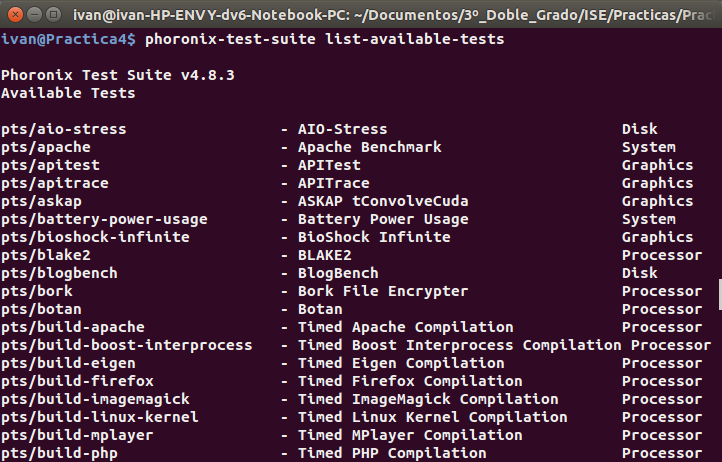
\includegraphics[width=0.7\linewidth]{phoronix-tests}
		\caption[phoronix-tests]{Lista de los benchmarks que tiene disponible phoronix}
		\label{fig:phoronix-tests}
	\end{figure}
	
	\item \textbf{Seleccione, instale y ejecute uno, comente los resultados.}\\
	El benchmark que hemos descargado es el que mide el uso de batería: $battery$-$power$-$usage$. Para instalarlo, ejecutamos el comando $install$ de phoronix. Para ejecutarlo utilizamos el comando $run$. Al ejecutarlo, se nos dice con que nombre queremos que se guarden los resultados. Tras esto, ejecuta el benchmark seleccionado. En nuestro caso, el benchmark mide el uso de la batería en sin hacer nada, con la pantalla apagada y reproduciendo un video. La gráfica que muestro el uso que ha hecho nuestro computador durante el mismo es el siguiente:\\
	\begin{figure}[H]
		\centering
		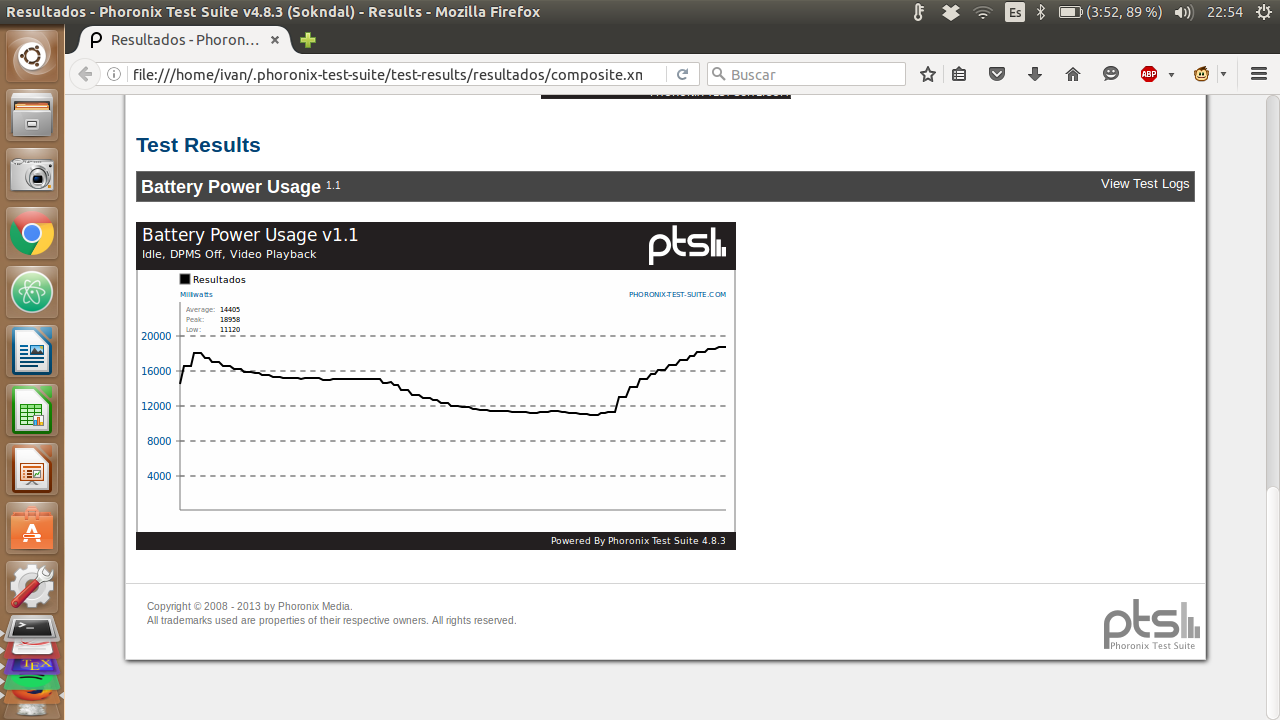
\includegraphics[width=0.7\linewidth]{Grafico_resultados_phorenix}
		\caption[Grafico benchmark]{Gráfica que muestra el uso de batería durante el benchmark en MiliWatios.}
		\label{fig:Grafico_resultados_phorenix}
	\end{figure}


\end{itemize}

\subsection{Tests de estrés para Webs.}
\subsubsection{Apache Benchmarck}
En este apartado vamos a responder las preguntas relacionadas con Apache Benchmark(comando ab).\\
\begin{itemize}
	\item \textbf{De los parámetros que le podemos pasar al comando ¿Qué significa -c 5 ? ¿y -n 100? Monitorice la ejecución de ab contra alguna máquina (cualquiera) ¿Cuántos procesos o hebras crea ab en el cliente?}\\
	Según la documentación oficial de Apache(la reference al comando ab) \cite{ab}, la opción -$n$ $request$ fija el número de peticiones que se harán al servidor de apache a $request$. La opción -c, a su vez, fija el número de peticiones concurrentes que dejaremos hacer al cliente. \\
	Tras esta explicación, vayamos ahora a monitorizar un equipo. Para ello, desde la máquina cliente ejecutamos el siguiente comando para bombardear a peticiones nuestro servidor:\\
	
	ab -n 1000 -c 10 http://10.0.2.6/\\
	
	el cual envía 1000 peticiones a través de 10 hebras paralelas(peticiones concurrentes). Este es el resultado de nuestro Benchmarking:\\
	
	\begin{figure}[H]
		\centering
		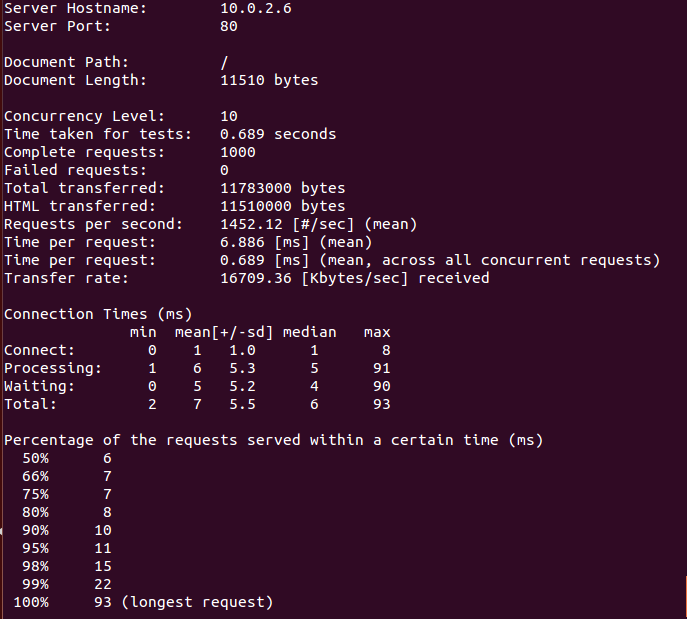
\includegraphics[width=0.7\linewidth]{Ejecucion-ab}
		\caption[Ejecucion ab]{Resultados obtenidos a través del comando ab}
		\label{fig:Ejecucion-ab}
	\end{figure}
	
	Estos resultados nos resumen cuanto ha tardado el servidor en atender a cada petición. A primera vista, nos llama la atención que la diferencia entre el máximo y el mínimo tiempo tardado en dar respuesta a las peticiones es muy grande(90 ms). Si nos fijamos en las últimas filas de la terminal, nos damos cuenta que esto es por la existencia de casos extremos, en los que solo el 1\% de las peticiones ha tardado entre 90 y 22 ms. Todas las demás no han llegado a tardar 22 ms.
	
	\item \textbf{Ejecute ab contra las tres máquinas virtuales (desde el SO anfitrión a las máquina virtuales de la red local, en Ubuntu, CentOS y WS) una a una (arrancadas por separado) y muestre y comente las estadísticas. ¿Cuál es la que proporciona mejores resultados? Fíjese en el número de bytes transferidos, ¿es igual para cada máquina?}\\
	
	Vamos a bombardear a cada máquina con las mismas peticiones y el mismo límite de concurrencia. Vamos a lanzar 1000 peticiones con, como mucho, 10 peticiones a la vez.\\
	
	La primera máquina a la que vamos a bombardear con peticiones es Windows. Estos son los resultados:\\
	\begin{figure}[H]
		\centering
		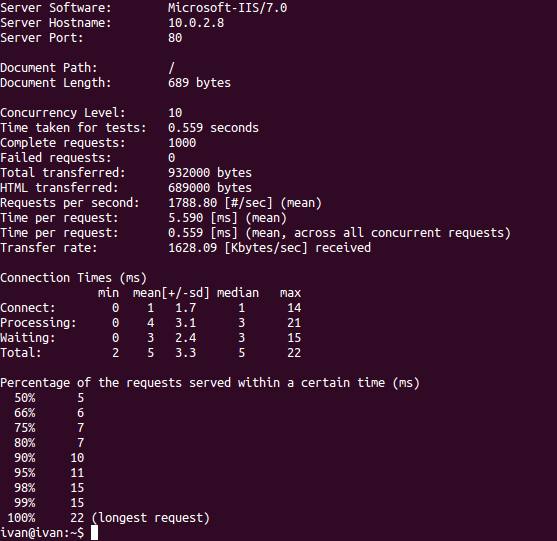
\includegraphics[width=0.6\linewidth]{Windows-ab}
		\caption[Windows ab]{Resultados del bombardeo de peticiones a Windows}
		\label{fig:Windows-ab}
	\end{figure}
	
	La siguiente máquina a bombardear es Ubuntu. Estos son los resultados:\\
	\begin{figure}[H]
		\centering
		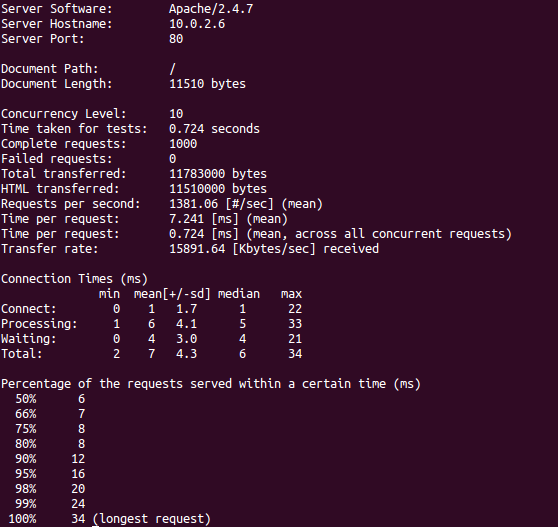
\includegraphics[width=0.6\linewidth]{Ubuntu-ab}
		\caption[Ubuntu-ab]{Resultados del bombardeo de peticiones a Ubuntu}
		\label{fig:Ubuntu-ab}
	\end{figure}
	La última máquina a bombardear es CentOs. Estos son los resultados:\\
	\begin{figure}[H]
		\centering
		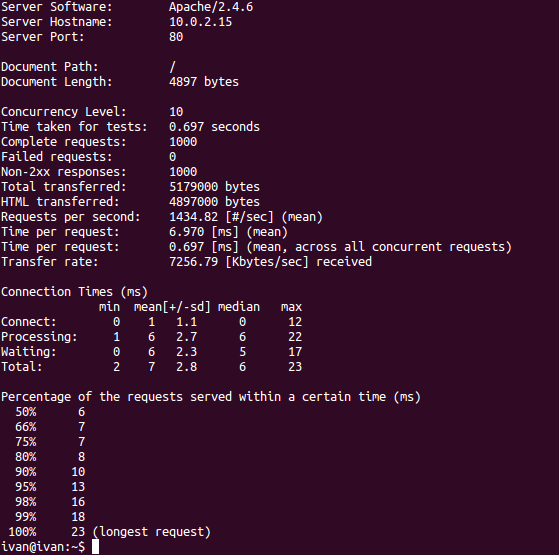
\includegraphics[width=0.6\linewidth]{CentOS-ab}
		\caption[CentOS ab]{Resultados del bombardeo de peticiones a CentOS}
		\label{fig:Centos-ab}
	\end{figure}
	
	En cada informe, nos dice la cantidad de información que se envía. En este caso, Ubuntu manda mucha información(11.510B de información), Windows envía sólo 689B de información y CentOs, 4.897B. Esto desencadena en que, obviamente, la velocidad que tardará Ubuntu en servir la página será mayor que las otras dos distribuciones, ya que la página en cuestión es más pesada.\\
	Como venimos anunciando, Ubuntu ha tardado más en servir las 1000 peticiones(0.724 seg), seguido muy de cerca, sorprendentemente, por Windows(0.559 seg). CentOS, por el contrario, ha tardado sólo 0.097 seg.\\
	
	
\end{itemize}

\subsubsection{Gatling}
\begin{itemize}
	\item \textbf{¿Qué es Scala? Instale Gatling y pruebe los escenarios por defecto.}\\
	Scala \cite{scala} es un lenguaje de programación que use los conceptos de orientación a objetos y los funcionales, formando un lenguaje multiparadigma. Está diseñado para expresar patrones de programación y es altamente tipado.\\
	Tras esta explicación, veamos ahora cómo usar la herramienta gatling para estresar el sistema. Según la guia de inicio rápido suministrada por el proyecto gatling \cite{gatling}, para instalar el programa simplemente hay que descomprimir un archivo que te descargas de la misma página para tener el programa en funcionamiento. En el directorio $./bin$ se encuentran los ejecutables de la aplicación. Para correr la aplicación, ejecutamos el ejecutable $./bin/gatling.sh$(en Linux) y nos saldrá una muestra de los tests de ejemplo. El que nosotros ejecutaremos será el test básico. Al terminar, nos dirá que para ver los resultados abramos un link creado en el directorio $./results$. Una de las tablas que crea gatling es la siguiente, donde muestra lo que tarda el sistema en responder a una query de la base de datos.\\
	\begin{figure}[H]
		\centering
		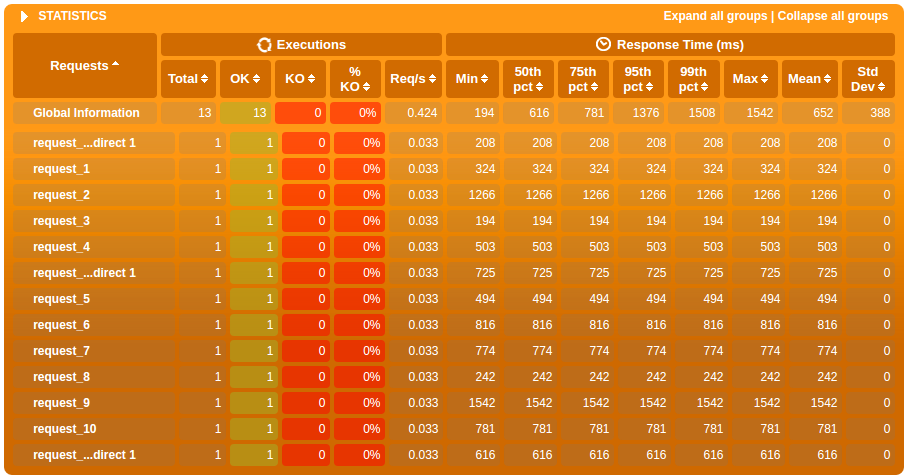
\includegraphics[width=0.7\linewidth]{Gatling_results1}
		\caption[Table resultados]{Tabla de resultados del test de estrés donde gatling mide lo que tarda el sistema en responder a una petición.}
		\label{fig:Gatling_results1}
	\end{figure}
	
	Y aquí los gráficos generados:\\
	\begin{figure}[H]
		\centering
		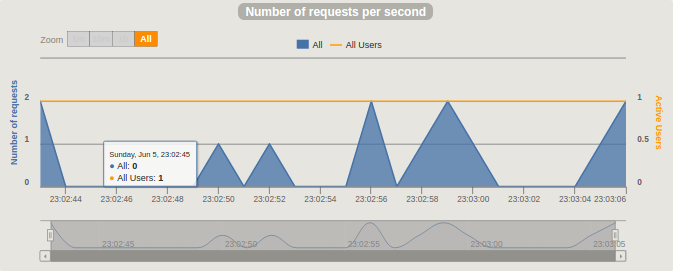
\includegraphics[width=0.7\linewidth]{NumeroRequestGatling}
		\caption[Peticiones por segundo]{Gráfico que muestra el número de peticiones por segundo en el transcurso del test.}
		\label{fig:NumeroRequestGatling}
	\end{figure}
	\begin{figure}[H]
		\centering
		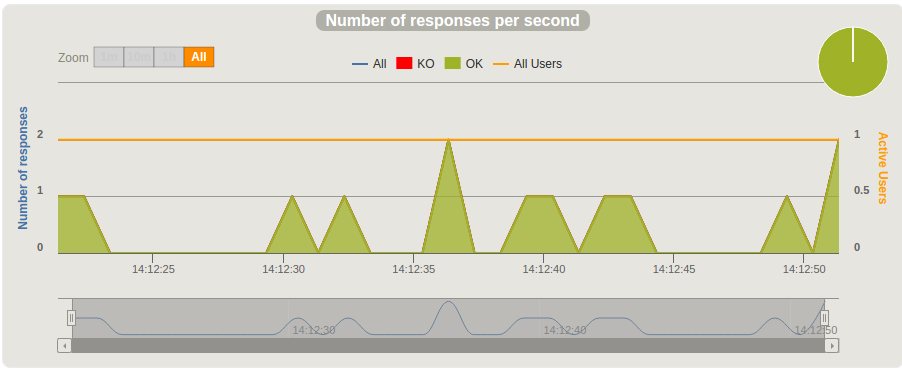
\includegraphics[width=0.7\linewidth]{NumeroRespuestasGatling}
		\caption[Respuestas gatling]{Gráfico que muestra el número de respuestas por segundo en el transcurso del test.}
		\label{fig:NumeroRespuestasGatling}
	\end{figure}
	
\end{itemize}
\subsubsection{Jmeter}
\begin{itemize}
	\item \textbf{Lea el artículo y elabore un breve resumen\cite{benchmarkingJmGt}.}\\
	El artículo pretende poner cara a cara las prestaciones de la herramienta vista anteriormente(Gatling) y Jmeter, una herramienta parecida. Al inicio del artículo deja muy claro que no quieren poner una por encima de la otra, ya que no es la intención de la página(flood.io), que apoya a ambas, eliminar una en función de la otra. Esto es porque piensan que estas herramientas necesitan distintos requerimientos.\\
	
	Los primeros párrafos describen en que circunstancias se van a llevar a cabo las pruebas con ambas herramientas y por qué. Utilizan, por ejemplo, un servidor con 4 CPUs virtuales en el que han habilitado 15 GB de RAM para asegurarse de que no se producen cuellos de botella en el servidor. También se dejan claros otros detalles, como que se correrá sobre la máquina virtual de Java con una serie de opciones de la misma(aquí no especificadas).\\
	
	La rutina que seguirá el benchmark consistirá en distintas transacciones hechas por "usuarios", cada una de ellas con distintos requerimientos usando recursos mas o menos lentos para tener una idea de todos los tipos de peticiones que se pueden hacer. \\
	
	Los últimos parámetros que se tienen en cuenta son la cantidad de peticiones, el nivel de concurrencia y el tiempo del mismo benchmark. Se correrán 10.000 hebras usuario, 30.000 peticiones por minuto y se correrá durante 20 minutos, con un tiempo de descanso de la máquina de 10 minutos.\\
	
	En este test, puesto que hay varias versiones de Jmeter, se ha pasado a medir las prestaciones de una y otra versión. Nosotros solo evaluaremos la diferencia que hay entre las dos herramientas(Gatling y Jmeter) no entre las distintas versiones de Jmeter.\\
	
	A continuación, pasamos a describir los resultados:\\
	
	\begin{itemize}
		\item Para empezar, la media que calculaba cada uno de los tests era muy parecida, al igual que la desviación típica, por tanto podemos coincidir en que se obtienen casi los mismos resultados con ambos testers.
		\item
		\item
		\item
		\item
		\item
	\end{itemize}
	
	 
\end{itemize}



\newpage

\begin{thebibliography}{xx}
	\bibitem{phoronix} http://www.phoronix-test-suite.com/documentation/phoronix-test-suite.pdf
	\bibitem{ab} https://httpd.apache.org/docs/2.4/programs/ab.html
	\bibitem{scala} http://www.scala-lang.org/
	\bibitem{gatling} http://gatling.io/docs/2.2.1/quickstart.html
	\bibitem{benchmarkingJmGt} https://blog.flood.io/benchmarking-jmeter-and-gatling/
	\bibitem{necesario}
	https://repo1.maven.org/maven2/io/gatling/highcharts/gatling-charts-highcharts-bundle/2.1.7/gatling-charts-highcharts-bundle-2.1.7-bundle.zip
	
\end{thebibliography}
\end{document}